\section{Integralrechnung}
In diesem Kapitel wird die Integralrechnung vorgestellt.
Die zentrale Theorie beinhaltet uneigentliche und bestimmte Integrale sowie die Techniken der partiellen Integration und der Substitution.


\subsection{Unbestimmtes Integral}

\index{Integral!unbestimmt}
\index{Integral!Konstante}
\index{Integral!Stammfunktion}
\begin{mybox}{Definition}
Wir bezeichnen eine Funktion $F(x)$ als 
\textit{Stammfunktion} der Funktion $f$,
falls $F^\prime(x) = f(x)$ gilt.\\
Ist $F$ eine Stammfunktion von $f$, so heißt
\begin{align*}
\int f(x) \td{x} = F(x) + C
\end{align*}
\textit{unbestimmtes Integral} von $f$.
Hierbei ist $C \in \mathbb{R}$ die \textit{Integrationskonstante}.
\end{mybox}

Die Ableitung einer Konstanten $C$ ist immer die Nullfunktion.
Aus diesem Grund gibt es unendlich viele Stammfunktionen $F$ zu einer Funktion $f$.
Man kann bei
\begin{align*}
\int f(x) \td{x} = F(x) + C
\end{align*}
auch von einer Menge an Funktionen sprechen.
\\
\index{Integral!Linearität}
\begin{mybox}{Linearität des Integrals}
Für Funktionen $f$, $g$ und $\alpha \in \mathbb{R}$
gilt:
\begin{enumerate}
\item 
$\int f(x) + g(x) \td{x} = \int f(x)  \td{x} + \int  g(x) \td{x}$
\item 
$\int \alpha \cdot f(x) \td{x} = \alpha \cdot\int  f(x) \td{x}$
\end{enumerate}
\end{mybox}
\ \\
Diese Eigenschaft vereinfacht das Berechnen von Stammfunktionen.
Um das Integral 
\begin{align*}
\int 2x^2 + x^3 \td{x}  = 2 \int x^2  \td{x}  + \int x^3 \td{x} 
\end{align*}
zu berechnen, wenden wir die Linearität des Integrals an. Wir sehen hieran, dass konstante Faktoren ignoriert und Summanden einzeln integriert werden können.\\
\\
Um Stammfunktionen von komplexeren Funktionen zu berechnen, genügt es oft, einige elementare Stammfunktionen zu kennen.\\
\newpage
\textbf{Elementare Stammfunktionen:}\index{Integral!Stammfunktion}
\begin{enumerate}
\item 
$\int 1 \td{x} = x + C$
\item
$\int x \td{x} = \frac{1}{2} \cdot x^2 +C$
\item
$\int x^2 \td{x} = \frac{1}{3} \cdot x^3 + C$ 
\item
$\int x^n \td{x} = 
\frac{1}{n+1} \cdot x^{n+1}+ C , \ n \neq -1
$
\item
$\int \frac{1}{x} \td{x} = \ln(x) + C$
\item $\int e^x \td{x} = e^x + C$
\item $\int \sin(x) \td{x} = - \cos(x) + C$
\item $\int \cos(x) \td{x} = \sin(x) +C$
\end{enumerate}
Um komplizierte Integrale zu lösen, wendet man häufig die Konzepte der partiellen Integration und der Substitution an.
Diese werden wir in den weiterführenden Abschnitten behandeln.

\newpage

\subsection{Bestimmtes Integral}
%\begin{tikzpicture}
%   \begin{axis}[axis lines=middle,samples=1000,no marks,,xlabel={$x$},
%ylabel={$y$}]
%        \addplot+[smooth,name path = A ] coordinates { (1,0.5) (2,1) (3,0.5) (4,0.7) (5,0.4) (6,0.3) };
%        %\addplot+[gray] fill between[of=A and B,soft clip={domain=2.5:5}];
%    \end{axis}
%\end{tikzpicture}
\index{Integral!bestimmt}
\begin{mybox}{Definition}
Mit dem \textit{bestimmten Integral} 
\begin{align*}
\int \limits_a^b f(x) \td{x}
\end{align*}

wird die Fläche zwischen der $x$-Achse und dem Funktionsgraph $f(x)$ mit den Integrationsgrenzen $a$ und $b$
\begin{center}
%\begin{tikzpicture}[scale=1.0,transform shape]
%% the initial drawing
%\draw[->] (-0.3,0) -- (5,0) node[right] {$x$} coordinate (x axis);
%\draw[->] (0,-0.3) -- (0,3) node[above] {$y$};
%\draw [name path=curve] (0.5,2) .. controls (1.5,2.8) and (3.5,1) .. (4.5,2);
%\path [name path=line 1] (1,0) -- (1,3);
%\path [name path=line 2] (4,0) -- (4,3);
%\path [name intersections={of=curve and line 1, by={a}}];
%\path [name intersections={of=curve and line 2, by={b}}];
%\path[name path=bottom] (1,0) --(4,0);
%\draw (1,0) node[below] {$a$} -- (a);
%\draw (4,0) node[below] {$b$} -- (b);
%\node[above=10pt] at (b) {$y=f(x)$};
%
%\end{tikzpicture}
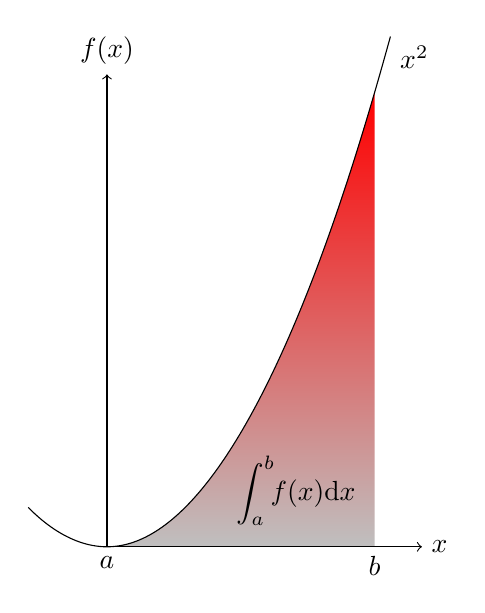
\begin{tikzpicture}[scale=2]
  \shade[top color=red,bottom color=gray!50] 
      (0,0) parabola (1.7,2.89) |- (0,0);
  \draw (1.2cm,2pt) node[above] 
      {$\displaystyle\int_a^b \!\!f(x)\mathrm{d}x$};

  \draw[->] (0,0) -- (2,0) node[right] {$x$};
  \draw[->] (0,-0) -- (0,3) node[above] {$f(x)$};
	\draw (0,0) node[below] {$a$} -- (0,0);
\draw (1.7,0) node[below] {$b$} -- (1.7,0);

  \draw (-.5,.25) parabola bend (0,0) (1.8,3.24) node[below right] {$x^2$};
\end{tikzpicture}
\end{center}

beschrieben.
\end{mybox}
\ \\
Das bestimmte Integral ist im Gegensatz zum unbestimmten Integral eine Zahl.
Die Berechnung führen wir jedoch auf unbestimmte Integrale zurück.\\
\index{Integral!Hauptsatz}
\begin{mybox}{Hauptsatz der Integralrechnung}
Sei $F$ eine Stammfunktion der Funktion $f$ und $a \leq b$.
Dann gilt:
\begin{align*}
\int \limits_a^b f(x) \td{x} = F(x) + C \bigg|_a^b = F(x)  \bigg|_a^b = F(b) - F(a)
\end{align*}
\end{mybox}
\ \\
Wir werten also die Stammfunktion an den Integrationsgrenzen aus und erkennen, dass die Integrationskonstante hier keine Rolle spielt.
Für das bestimmte Integral gelten dieselben Eigenschaften wie für das unbestimmt Integral.
\newpage
\textbf{Weitere Eigenschaften:}\\
Sei $f$ eine Funktion.
\begin{enumerate}
\item Für $a \leq c \leq b$ gilt
\begin{align*}
\int \limits_a^b f(x) \td{x} = \int \limits_a^c f(x) \td{x} + \int \limits_c^b f(x) \td{x}.
\end{align*}

\item 
Für beliebige $a,b \in \mathbb{R}$ gilt
\begin{align*}
\int \limits_a^{\textcolor{red}{b}} f(x) \td{x}
= 
- \int \limits_{\textcolor{red}{b}}^a f(x) \td{x}.
\end{align*}
\end{enumerate}

Die erste Eigenschaft ist notwendig, um abschnittsweise definierte Funktionen zu integrieren.
Gegeben sei die Funktion 
\begin{align*}
f(x) 
= 
\begin{cases}
&x  , \ \text{falls} \ 0 \leq x < 1\\
&1  , \ \text{falls} \ 1 \leq x \leq 2
\end{cases}.
\end{align*}
Dann gilt 
\begin{align*}
\int \limits_0^2 f(x) \td{x}
= \int \limits_0^1 f(x) \td{x} + \int \limits_1^2 f(x) \td{x}
= \int \limits_0^1 x \td{x} + \int \limits_1^2 1 \td{x} 
= \frac{1}{2}\cdot 1^2 - \frac{1}{2} \cdot 0^2 + 2 - 1 
= \frac{1}{2  } + 1 = \frac{3}{2}
\end{align*}
durch Anwenden der ersten Eigenschaft.
Die zweite Eigenschaft findet hauptsächlich Anwendung, wenn die untere Grenze größer als die obere ist.
Dadurch kann man auf diese Integrale den Hauptsatz anwenden.
Dies lässt sich beispielsweise durch
\begin{align*}
\int \limits^0_1 x \td{x} = - \int \limits^1_0 x \td{x} = -\frac{1}{2} x^2 \bigg|_0^1 
= - \left( \frac{1}{2} \cdot 1^2 - \frac{1}{2} \cdot 0^2\right)  
= -\frac{1}{2} 
\end{align*}
veranschaulichen.\\
\\
\subsubsection*{Anwendungsbeispiel A}

Wir betrachten:
\begin{align*}
\int \limits_0^{2\pi} \cos(x) \td{x}
= 
\sin(x) \bigg|_0^{2\pi} = \sin(2\pi) - \sin(0) = 0 -0 = 0
\end{align*}
Dieses Integral müssen wir eigentlich nicht berechnen.
Dies könntest du dir an einer Skizze veranschaulichen.
\begin{center}
	\includegraphics[scale=0.15]{sections/pics/Sine_cosine_one_period}
\end{center}

\subsubsection*{Anwendungsbeispiel B}
$\int \limits_1^e \frac{1}{x} \td{x}
= \ln(x) \bigg|_1^e = \ln(e) - \ln(1) = 1$. 

\subsubsection*{Anwendungsbeispiel C}
Nun interessieren wir uns für die die Integration von abschnittsweise definierten Funktionen, dass heißt:
\begin{align*}
f:[x_0,x_k] \to \mathbb{R}, \quad
f(x)
= 
\begin{cases}
g_1(x) &, \text{ für } x_0 \leq x < x_1 \\
g_2(x) &, \text{ für } x_1 \leq x < x_2\\
\vdots  &\ \\
g_k(x) &,  \text{ für } x_{k-1} \leq x < x_k
\end{cases}
\end{align*}
Funktionen dieser Art integrieren wir mit Eigenschaft 1 abschnittsweise:
\begin{align*}
\int \limits_{x_0}^{x_k} f(x) \td{x}
= \sum \limits_{i=1}^k \int \limits_{x_{i-1}}^{x_i} g_i(x) \td{x}
\end{align*}
Dieses Beispiel ist zunächst abstrakt.
Wir betrachten die Betragsfunktion
\begin{align*}
| \cdot | : \mathbb{R} \to [0,\infty) 
, \quad
x \mapsto 
\begin{cases}
x, &\ \text{falls } x \geq 0\\
-x, &\ \text{falls }  x < 0
\end{cases}.
\end{align*}
Hierbei symbolisiert $|\cdot |$ das Einsetzen von $x$-Werten für den Punkt.
Dann gilt:
\begin{align*}
\int \limits_{-1}^1 |x| \td{x}
&= \int \limits_{-1}^0 |x| \td{x}
+ \int \limits_{0}^1 |x| \td{x}
=\int \limits_{-1}^0 -x \td{x}
+ \int \limits_{0}^1 x \td{x}\\
&=
- \frac{1}{2} x^2 \bigg|_{-1}^0 + \frac{1}{2} x^2 \bigg|_{0}^1
=
-\left(\frac{1}{2} \cdot 0^2 - \frac{1}{2} \cdot  (-1)^2 \right)
+
\frac{1}{2} \cdot 1^2 - \frac{1}{2} \cdot 0^2
= \frac{1}{2} + \frac{1}{2} = 1
\end{align*}


\newpage

\subsection{Partielle Integration}
Die partielle Integration findet Anwendung, wenn
wir die zu integrierende Funktion als Produkt schreiben können.
Hierzu betrachten wir die Produktregel der Differenzialrechnung
\begin{align*}
(u(x) \cdot v(x))^\prime = u^\prime(x) v(x) + u(x) v^\prime(x)
\end{align*}
und wenden auf beiden Seiten das unbestimmte Integral an.
Dadurch erhalten wir mit
\begin{align*}
\textcolor{blue}{\int (u(x) \cdot v(x))^\prime \td{x}}
&=
\textcolor{green}{\int u^\prime(x) v(x) \td{x}} 
 + 
 \textcolor{red}{\int u(x) v^\prime(x)\td{x}}
 \\
\Leftrightarrow
\textcolor{green}{\int u^\prime(x) v(x) \td{x}}  &= \textcolor{blue}{\int (u(x) \cdot v(x))^\prime \td{x}} - \textcolor{red}{\int u(x) v^\prime(x)\td{x}}
= u(x) \cdot v(x) - \int u(x) v^\prime(x)\td{x}
\end{align*}
eine Rechenvorschrift zum Berechnen von Funktionen der Form $f(x) = u^\prime(x) v(x)$.
Die gleichen Rechnungen lassen sich auch mit bestimmten Integralen wiederholen.\\
\index{Integral!partielle Integration}
\begin{mybox}{Partielle Integration}
Seien $u, v$ Funktionen.
Dann gilt:
\begin{enumerate}
\item
$\int u^\prime(x) \cdot v(x) \td{x} = u(x) \cdot v(x) - \int u(x) v^\prime(x)\td{x} $
\item
$\int \limits_a^b u^\prime(x) \cdot v(x) \td{x} = u(x) \cdot v(x) \bigg|_a^b - \int \limits_a^b u(x) v^\prime(x)\td{x} $
\end{enumerate}
\end{mybox}
\ \\
Wir erkennen, dass diese Regel gleichermaßen für unbestimmte und bestimmte Integrale gilt.
Jedoch ist es häufig übersichtlicher zunächst die Stammfunktion mit partieller Integration zu bestimmen und dann den Hauptsatz anzuwenden.\\
\\
Durch partielle Integration lassen sich nun auch geschickt neue Stammfunktionen finden.
Wir betrachten 
\begin{align*}
\int \ln(x) \td{x} = 
\int\underbrace{ 1 \cdot \ln(x)v}_{u^\prime(x) \cdot v(x)}\td{x} 
= \underbrace{x \cdot \ln(x)}_{u(x) \cdot v(x)} - \int \underbrace{ x  \cdot \frac{1}{x}}_{u(x) \cdot v^\prime(x)} \td{x}= x \ln(x) -x + C
\end{align*}
mit $u^\prime(x) = 1 $ und $v(x) = \ln(x) $.
Nützlich ist die partielle Integration, wenn wir ein Produkt aus einer leicht integrierbaren Funktion und einer Funktion deren Ableitung nach endlichen vielen Ableitungen Null ergibt, haben.
Dies kann man sich an folgenden Integralen veranschaulichen:
\begin{align*}
&\int \limits_a^b x \cdot e^x \td{x}\\
&\int \limits_a^b x^{20} \sin(x) \td{x}\\
&\int \limits_a^b x^{1000} \cos(x) \td{x}
\end{align*}
Die erste Funktion ergibt Null nach endlich vielen Ableitungen.
Wir müssen nur lange genug Ableiten, damit die Funktion konstant wird.
Von den zweiten Funktionen kennen wir immer die Stammfunktion.
Die obigen Integrale lassen sich aus diesem Grund geschickt mit partieller Integration bestimmen, auch wenn wir die letzten beiden nicht von Hand ausrechnen wollen.

\subsubsection*{Anwendungsbeispiel}
Ein Investment Fonds generiert innerhalb der Zeitspanne von $t=0$ zu $T=12$ einen
stetigen Cashflow von $B(t) = 10 t + 5$.
Die Verzinsung erfolgt kontinuierlich zum Zinssatz $i = 5 \%$.
\\
\\
Bestimmen Sie den Nettobarwert $PV(0)$ zum Zeitpunkt $t = 0$ \textit{aller} Zahlungsströme,
die der Investment Fonds zwischen den Zeitpunkten $t = 0$ und $T = 12$ generiert.\\
\\
\textbf{Lösung:}
\begin{mdframed}
\underline{\textbf{Vorgehensweise:}}
\begin{enumerate}
\item Formuliere das Problem mathematisch.
\item Bestimme die nötige Stammfunktion mithilfe partieller Integration.
\item Berechne den Wert des Integrals.
\end{enumerate}
\end{mdframed}

\underline{1. Formuliere das Problem mathematisch}\\
Um den Nettobarwert $PV(0)$ zu bestimmen, müssen wir das Integral
\begin{equation*}
PV(0)
=
\int \limits_0^T B(t) e^{-i t} \ dt
=
\int \limits_0^{12} (10 t + 5) e^{-0.05 t} \ dt
\end{equation*}
berechnen.\\
\\
\underline{2. Bestimme die nötige Stammfunktion mithilfe partieller Integration}\\
%Zunächst betrachten wir die Produktregel und formen diese durch
%\begin{equation*}
%(u(t) v(t))^\prime = u^\prime(t) \cdot v(t) + u(t) \cdot v^\prime(t)
%\Leftrightarrow
%u(t) v^\prime(t) = (u(t)  v(t))^\prime - u^\prime(t) v(t)
%\end{equation*}
%um. Nun erhalten wir mit
%\begin{equation*}
%\int u(t) v^\prime(t) \ dt 
%= 
%\int (u(t)  v(t))^\prime \ dt - \int u^\prime(t) v(t) \ dt
%=
%u(t) v(t) - \int u^\prime(t) v(t) \ dt
%\end{equation*}
%die Regel für partielle Integration für unbestimmte Integrale.
%Für bestimmte Integrale geht die Umformung genauso.
%Dies war eine kurze Herleitung der partiellen Integration.
%Nun wenden wir diese Regel an.
Wir nutzen die Regel der partiellen Integration
\begin{align*}
\int u^\prime(t) \cdot v(t) \td{t} = u(t) \cdot v(t) - \int u(t) v^\prime(t)\td{t}
\end{align*}
und wählen hierfür
\begin{equation*}
\begin{split}
u^\prime(t)  =  e^{-0.05 t},  \quad
v(t)  = 10 t +5.
\end{split}
\end{equation*}
%für die partielle Integration.
Dies macht Sinn, denn $v$ wird nach einmal Ableiten konstant.
Es gilt 
\begin{equation*}
\begin{split}
u(t) = \frac{1}{-0.05} e^{-0.05t} 
=- \frac{100}{5} e^{-0.05t} = -20 e^{-0.05t}, \quad
v^\prime(t) = 10.
\end{split}
\end{equation*}
Mithilfe der Regel für partielle Integration erhalten wir
\begin{equation*}
\begin{split}
\int e^{-0.05 t} (10 t + 5)  \ dt
&= 
  -20  e^{-0.05 t} (10t +5)  - \int   -20 e^{-0.05t} \cdot 10  \ dt\\
&= -( 200 t + 100) e^{-0.05 t} + 200 \int e^{-0.05 t} \ dt\\
&=-(200 t + 100)  e^{-0.05t } + 200 (-20) e^{-0.05 t}  + C\\
&= -(200 t + 100) e^{-0.05 t } -4000 e^{-0.05t} + C \\
&= -(200 t +4100) e^{-0.05 t} + C
\end{split}
\end{equation*}
als Stammfunktion.\\

\newpage
\underline{3. Berechne den Wert des Integrals}\\
Da wir nun die Stammfunktion kennen, können wir das Integral direkt durch
\begin{align*}
\int \limits_0^{12} (10t + 5) e^{-0.05 t} \ dt
&=  \left[ -(200 t +4100) e^{-0.05 t} \right]_0^{12}\\
&= -(200 \cdot 12 +4100) e^{-0.05 \cdot 12} - (-(200 \cdot 0 +4100) e^{-0.05 \cdot 0} ) 
= -6500 e^{-0.6 }+4100 
\approx 532.70
\end{align*}
berechnen.\\
\\
Der Nettobarwert beträgt ungefähr $532.70$.

\newpage
\subsection{Integration durch Substitution}
\index{Integral!Substitution}
\begin{mybox}{Substitutionsregel}
Sei $f$ stetig und $g$ stetig differenzierbar.
Dann gilt:
\begin{align*}
\int \limits_a^b f( g(x)) \cdot g^\prime(x) \td{x} = 
\int \limits_{g(a)}^{g(b)} f(t) \td{t}
\end{align*}
Die Formel gilt analog für uneigentliche Integrale, nur eben ohne Grenzen.
\end{mybox}
Wir sehen bereits, dass $t = g(x) $ gelten muss.
Aber es ist noch nicht klar, wie $g^\prime(x)$ auf der rechten Seite verschwindet.
Hierfür schauen wir uns Folgendes an:
\begin{align*}
t = g(x) 
\Rightarrow
\frac{\mathrm{d} t}{\mathrm{d} x} = g^\prime(x) 
&\Leftrightarrow
\mathrm{d} t = g^\prime(x) \cdot \mathrm{d} x\\
&\Leftrightarrow
\mathrm{d} x = \frac{1}{g^\prime(x) } \cdot \mathrm{d} t
\end{align*}
Diese Umformungen geben uns zwei gleichwertige Möglichkeiten, die Substitution durchzuführen.
Die Erste ist $g^\prime(x)  \td{x} $ durch $\mathrm{d} t$ zu ersetzen.
Die Zweite ist, $\mathrm{d} x$ durch $\frac{1}{g^\prime(x) } \ \mathrm{d} t$ zu ersetzen.
Dadurch kürzt sich der $g^\prime(x)$ Term raus.\\ \\
Am einfachsten ist es die Substitution an Anwendungsaufgaben zu verstehen.
\newpage
\subsubsection*{Anwendungsbeispiel A}
Wir betrachten das Integral
\begin{align*}
\int \frac{2 x}{x^2} \td{x}
= 
\int \frac{1}{x^2} \cdot  2x \td{x}.
\end{align*}
Dann ist $f(x) = \frac{1}{x}$ und $g(x)=x^2$.
Wir können also 
\begin{align*}
\int \frac{1}{x^2} \cdot  2x \td{x} 
= 
\int f(g(x)) \cdot g^\prime(x)  \td{x}
\end{align*}
schreiben.
Wegen
\begin{align*}
t = g(x) = x^2 
\Rightarrow
\frac{\mathrm{d} t }{\mathrm{d} x}
= 
2 x 
\Leftrightarrow
\mathrm{d} t = 2x \ \mathrm{d} x
\end{align*}
können wir durch
\begin{align*}
\int \frac{1}{x^2} \cdot  2x \td{x}  = \int \frac{1}{t}  \td{t}  = \ln(t) +C =\ln(x^2) + C
\end{align*}
die Stammfunktion angeben.\\ \\
\textit{Wichtig:} Im letzten Schritt wurde rücksubstituiert.
Dies ist beim Berechnen von unbestimmten Integralen notwendig.
Bei bestimmten Integralen müssen wir dies nicht mehr machen.\\
Wir betrachten noch das ähnliche Integral
\begin{align*}
\int \frac{x}{x^2} \td{x} = \int \frac{1}{x^2} \cdot x \td{x}.
\end{align*}
Uns fällt auf, dass dieses Integral nicht die Form
\begin{align*}
\int f(g(x)) \cdot g^\prime(x)  \td{x}
\end{align*}
besitzt.
Zum Glück ist dies kein Problem.
Wir substituieren $t = x^2$.
Dann gilt wieder:
\begin{align*}
\frac{\mathrm{d} t }{\mathrm{d} x} = 2x 
\Leftrightarrow
\mathrm{d } x = \frac{1}{2 x} \td{t } = \frac{1}{2} \cdot \frac{1}{x} \td{t}
\end{align*}
Die weitere Rechnung werden wir nun so ausführlich wie möglich durchführen:
\begin{align*}
\int \frac{1}{x^2} \cdot x \td{x}
\stackrel{t = x^2}{=}
\int \frac{1}{t} \cdot x \td{x}
\stackrel{\mathrm{d } x = \frac{1}{2 x} \td{t }}{=}
\int \frac{1}{t} \cdot x \cdot \frac{1}{2x} \td{t}
= 
\frac{ 1}{2 } \cdot \int   \frac{1}{t} \td{t}
= 
\frac{1}{2} \cdot \ln(t) + C 
= 
\frac{1}{2} \cdot \ln(x^2) + C
\end{align*}
Was fällt uns auf?
Nach unserer Substitution hatten wir noch ein störendes $x$ im Integral.
Dieses kürzt sich jedoch mit $\mathrm{d} x = \frac{1}{2x} \mathrm{d}t$ heraus.
Der konstante Faktor interessiert uns beim Integrieren nicht. 
\newpage
\subsubsection*{Anwendungsbeispiel B}
Wir betrachten das bestimmte Integral
\begin{align*}
\int \limits_0^\pi \sin(\cos(x)) \cdot \sin(x) \td{x}.
\end{align*}

Wir substituieren $t = \cos(x)$.
Wegen
\begin{align*}
\frac{\mathrm{d} t}{\mathrm{d} x} = - \sin(x) 
\Leftrightarrow
\mathrm{d} x = -\frac{1}{\sin(x)} \td{t}
\end{align*}
erhalten wir 
\begin{align*}
\int \limits_0^\pi \sin(\cos(x)) \cdot \sin(x) \td{x}
= 
\int \limits_{\cos(0)}^{\cos(\pi)} \sin(t) \cdot \sin(x) \cdot \frac{-1}{\sin(x)} \td{t}
=
- \int \limits_{\cos(0)}^{\cos(\pi)} \sin(t)\td{t}
\end{align*}
als Integral. Bei bestimmten Integralen ist es notwendig, die Grenzen auch zu substituieren.
Mit 
\begin{align*}
\int \limits_0^\pi \sin(\cos(x)) \cdot \sin(x) \td{x}
&\stackrel{t = \cos(x)}{=}
- \int \limits_{\cos(0)}^{\cos(\pi)} \sin(t)\td{t}
=
- \int \limits_{1}^{-1} \sin(t)\td{t}
=
\int \limits_{-1}^{1} \sin(t)\td{t} \\ 
=
- \cos(t) \bigg|_{-1}^1 &= -\cos(1) + \cos(-1)
\stackrel{\text{a-symm.}}{=} -\cos(1) + \cos(1) = 0 
\end{align*}
erhalten wir den Wert des Integrals.
Hierbei haben wir die Achsensymmetrie der Kosinusfunktion verwendet.

\subsubsection*{Anwendungsbeispiel C}
Wir betrachten das Integral
\begin{align*}
\int \frac{f^\prime(x)}{f(x)} \td{x}.
\end{align*}
Mit $t = f(x) $ gilt
\begin{align*}
\frac{\mathrm{d} t}{\mathrm{d} x} = f^\prime(x)
\Leftrightarrow
\mathrm{d} t = f^\prime(x) \td{x}.
\end{align*}
Damit erhalten wir durch
\begin{align*}
 \int \frac{f^\prime(x)}{f(x)} \td{x}
 = 
 \int \frac{1}{t} \td{t} 
 =
 \ln(t) + C 
 =
 \ln(f(x)) + C
\end{align*}
eine allgemeine Stammfunktion für Funktionen der Form $\frac{f^\prime(x) }{f(x)}$.
Dies kann man direkt anwenden:
\begin{align*}
\int \frac{\cos(x)}{\sin(x)} \td{x} &= \ln(\sin(x)) +C \\
\int \frac{x}{ x^2} \td{x} &= \frac{1}{2} \int \frac{2x}{ x^2} \td{x} = \frac{1}{2} \ln(x^2) + C
\end{align*}

\newpage

\subsubsection*{Anwendungsbeispiel D}
Berechnen Sie das unbestimmte Integral
\begin{equation*}
\int \frac{\sin(\ln(x)) \ \cos(\ln(x))}{x} dx.
\end{equation*}
\textbf{Lösung:}
\begin{mdframed}
\underline{\textbf{Vorgehensweise:}}
\begin{enumerate}
\item Finde eine geeignete Substitution und bestimme die Stammfunktion.
\end{enumerate}
\end{mdframed}

\underline{1. Finde eine geeignete Substitution und bestimme die Stammfunktion}\\
Es gilt
\begin{equation*}
\frac{\text{d}}{\text{d} x}
\sin(\ln(x))
= \frac{\cos(\ln(x))}{x}
\end{equation*}
mit der Kettenregel.
Demnach haben wir durch
\begin{equation*}
\int \frac{\sin(\ln(x)) \ \cos(\ln(x))}{x} dx
=
\int \sin(\ln(x)) \cdot \frac{ \ \cos(\ln(x))}{x} dx
=
\int \sin(\ln(x)) \ \frac{\text{d}}{\text{d} x} \sin(\ln(x)) dx
\end{equation*}
die geeignete Substitution 
\begin{equation*}
u = \sin(\ln(x))
\end{equation*}
gefunden.
Durch 
\begin{equation*}
\frac{\text{d} u }{\text{d} x} = \frac{\cos(\ln(x))}{x}
\Rightarrow
\text{d}  u =  \frac{\cos(\ln(x))}{x} \ \text{d} x  
\end{equation*}
erhalten wir mit
\begin{equation*}
\int \frac{\sin(\ln(x)) \ \cos(\ln(x))}{x} dx 
=
\int u \ du
= \frac{1}{2} u^2 + C
= \frac{1}{2} (\sin(\ln(x)))^2 + C
\end{equation*}
die gesuchte Stammfunktion.\\ \\
Eine andere Möglichkeit ist, zweimal zu substituieren.
Zuerst substituieren wir $v = \ln(x)$.
Mit 
\begin{equation*}
\frac{\text{d} v}{\text{d} x}
= \frac{1}{x}
\Rightarrow
\text{d} v = \frac{1}{x} \ \text{d} x
\end{equation*}
erhalten wir
\begin{equation*}
\int \frac{\sin(\ln(x)) \ \cos(\ln(x))}{x} \ dx
= \int \sin(v) \cos(v) \ dv.
\end{equation*}
Die zweite Substitution ist $w = \sin(v)$.
Für diese gilt
\begin{equation*}
\frac{\text{d} w}{\text{d} v} = \cos(v)
\Rightarrow
\text{d} w = \cos(v) \ \text{d} v
\end{equation*}
und es folgt
\begin{equation*}
\begin{split}
\int \frac{\sin(\ln(x)) \ \cos(\ln(x))}{x} \ dx
&= \int \sin(v) \cos(v) \ dv
= \int w \ dw\\
&= \frac{1}{2} w^2 + C
= \frac{1}{2} (\sin(v))^2
= \frac{1}{2} (\sin(\ln(x)))^2 +C
\end{split}
\end{equation*}
durch zweimaliges Zurücksubstituieren.\\
\\
Die gesuchte Stammfunktion ist
\begin{align*}
\frac{1}{2} (\sin(\ln(x)))^2 +C.
\end{align*}

\subsection{Uneigentliches Integral}
Bisher haben wir nur Integrale von Funktionen betrachtet, welche auf beschränkten Intervallen definiert sind.
Doch wie sieht es aus, wenn Definitionslücken innerhalb der Integrationsgrenzen liegen oder die Grenzen $\pm \infty$ sind?
Wir können dies durch Grenzwerte auf bestimmte Integrale zurückführen.\\
\index{Integral!uneigentlich}
\begin{mybox}{Definition}
\begin{enumerate}
\item
Sei $f$ eine Funktion mit Definitionsbereich $D_f = [a,\infty)$, $D_f = (-\infty,b]$ oder $D_f = (-\infty, \infty)$.
Dann nennen wir 
\begin{align*}
\int\limits_a^\infty f(x) \td{x} &:= \lim  \limits_{\beta \to \infty} \int\limits_a^\beta f(x) \td{x}\\
\int\limits_{-\infty}^b f(x) \td{x} &:= \lim \limits_{\alpha \to \infty} \int\limits_{-\alpha}^b f(x) \td{x}\\
\int\limits_{-\infty}^{\infty} f(x) \td{x} &:=\lim \limits_{\alpha,\beta \to \infty} \int\limits_{-\alpha}^\beta f(x) \td{x}
\end{align*}
\textit{uneigentliche Integrale}, falls diese Grenzwerte existieren. 
\item
Sei $f$ eine Funktion mit Definitionslücke an der Stelle $b$.
Dann nennen wir
\begin{align*}
\int \limits_a^b f(x) \td{x} := \lim \limits_{\beta \to b} \int \limits_a^\beta f(x) \td{x} 
\end{align*}
\textit{uneigentliches Integral}, falls der Grenzwert existiert.
\end{enumerate}
\end{mybox}
Im Endeffekt läuft es darauf hinaus, dass wir wie gewohnt Stammfunktionen finden.
Wir müssen nur $\pm \infty$ Grenzen und Definitionslücken als Grenzwerte betrachten und überprüfen, ob diese Grenzwerte existieren.
\subsubsection*{Anwendungsbeispiel A}
Wir betrachten das Integral
\begin{align*}
\int \limits_0^1 \frac{1}{x^2} \td{x}.
\end{align*}
Warum ist dies uneigentlich? Die $0$ ist eine Definitionslücke von $\frac{1}{x^2}$.
Zunächst integrieren wir 
\begin{align*}
\int \limits_\alpha^1 \frac{1}{x^2} \td{x} = - \frac{1}{x} \bigg|_\alpha^1 =  -1 - \frac{-1}{\alpha}= -1 + \frac{1}{\alpha}
\end{align*}
mit $\alpha > 0$.
Wichtig ist hier, dass man nicht über die Definitionslücke laufen darf.
Nun gilt
\begin{align*}
\lim \limits_{\alpha \to 0}  \int \limits_\alpha^1 \frac{1}{x^2} \td{x}  = \lim \limits_{\alpha \to 0}  -1 + \frac{1}{\alpha} = \infty,
\end{align*}
womit der Grenzwert nicht existiert.
Damit ist 
\begin{align*}
\int \limits_0^1 \frac{1}{x^2} \td{x}.
\end{align*}
kein uneigentliches Integral.

\subsubsection*{Anwendungsbeispiel B}
Wir betrachten
\begin{align*}
\int \limits_1^\infty \frac{1}{x^2} \td{x}.
\end{align*}

Zunächst gilt
\begin{align*}
\int \limits_1^\beta \frac{1}{x^2} \td{x} = \frac{-1}{x} \bigg|_1^\beta = - \frac{1}{\beta} - (-1)
=
-\frac{1}{\beta } + 1
\end{align*}
womit wir durch
\begin{align*}
\lim \limits_{\beta \to \infty}  \int \limits_1^\beta \frac{1}{x^2} \td{x} 
= 
\lim \limits_{\beta \to \infty} - \frac{1}{\beta} + 1 = 1
\end{align*}
ein uneigentliches Integral gefunden haben.

\newpage
\subsection{Dichtefunktion}
\index{Dichtefunktion}
\begin{mybox}{Definition}
\index{Dichtefunktion}
Wir nennen eine Funktion $f$ \textit{Dichtefunktion} auf $I = [a,b] \subseteq \mathbb{R}$, falls
\renewcommand{\labelenumi}{(\roman{enumi})}
\begin{enumerate}
\item $f(x) \geq 0 $ für $x \in I$ 
\item $\int_I f(x) \td{x} =\int \limits_a^b f(x) \td{x}= 1$.
\end{enumerate}
erfüllt ist.
\end{mybox}

\subsubsection*{Anwendungsbeispiel A}
Die Funktion $f$ hat folgende Eigenschaften:
\renewcommand{\labelenumi}{(\roman{enumi})}
\begin{enumerate}
\item $f(x) \geq -3 $ für $x \in [0,1],$ und
\item $\int_0^1 f(x) dx = 3$.
\end{enumerate}
Dann gilt:
\renewcommand{\labelenumi}{(\alph{enumi})}
\begin{enumerate}
\item $g_1  =  \frac{1}{3} f $ ist eine Dichtefunktion auf $[0,1]$.
\item $g_2  =   f +3 $ ist eine Dichtefunktion auf $[0,1]$.
\item
$g_3  =  \frac{1}{6} f +3 $ ist eine Dichtefunktion auf $[0,1]$.
\item
$g_4  =  \frac{1}{6} f + \frac{1}{2} $ ist eine Dichtefunktion auf $[0,1]$.
\end{enumerate}
\ \\
Wir wissen, dass
\begin{align*}
g_1(x) = \frac{1}{3} f(x) \geq \frac{1}{3} (-3) = -1
\end{align*}
gilt.
Damit ist Antwort (a) falsch.\\
Für $g_2$ ist
\begin{align*}
g_2(x) = f(x) + 3 \geq -3 +3 = 0
\end{align*}
erfüllt. Jedoch ist die zweite Bedingung wegen
\begin{align*}
\int \limits_0^1 g_2(x) \ dx 
= 
\int \limits_0^1 f(x) + 3 \ dx
=
\int \limits_0^1 f(x) \ dx + \int \limits_0^1 3 \ dx
=
3 + 3 = 6
\end{align*}
nicht erfüllt.\\
Für $g_3$ ist wegen 
\begin{align*}
g_3(x) = \frac{1}{6} f + 3 \geq \frac{1}{6} \cdot (-3) +3
= -\frac{1}{2} +3 = \frac{5}{2}
\end{align*}
die erste Bedingung erfüllt.
Jedoch gilt
\begin{align*}
\int \limits_0^1 g_3(x) \ dx
= 
\frac{1}{6} \int \limits_0^1 f(x) \ dx + \int \limits_0^1 3 \ dx
= 
\frac{1}{6} \cdot 3 +  3 = \frac{1}{2} + 3 = \frac{7}{2}
\end{align*}
für die zweite Bedingung.
Also wissen wir schon durch das Ausschlußprinzip, dass Antwort (d) korrekt ist.
Die Funktion $g_4$ erfüllt beide Bedingungen:
\begin{align*}
g_4(x) &= \frac{1}{6} f(x) + \frac{1}{2}
= - \frac{1}{2} + \frac{1}{2} = 0\\
\int \limits_0^1 g_4(x) \ dx &=
\frac{1}{6} \int \limits_0^1 f(x) \ dx + \int \limits_0^1 \frac{1}{2} \ dx
= \frac{1}{2} + \frac{1}{2} = 1
\end{align*}
\ \\
Die Antwort (d) ist korrekt.